\documentclass[12pt,oneside,a4paper]{article}
\usepackage[nosumlimits]{amsmath}
\usepackage{graphicx} 
\usepackage{amsmath}
\begin{document}
\title{\Large{\textbf{Hochschule München\\ 
Studiengang Informatik\\ 
\bigskip
\bigskip
\bigskip
\bigskip
\bigskip
\bigskip
Angewandte Mathematik\\
Übungsblatt 2}}}
\bigskip
\author{Bastian Kersting,
Michael Schober,
Elena Lilova
IF2B}
\maketitle
\newpage
\begin{center}
\LARGE
 \textbf{Aufgabe 1} 
\bigskip
\bigskip
\end{center}
\begin{flushleft}
Ziel der ersten Aufgabe ist die Summe einer Komplexen Zahl mit Benutzung der Polarform der komplexen Zahl zu berechnen: $$
\sum_{k=0}^{30} (1.1 - 02.i)^k $$ 
Zur Berechnung der Summe haben wir Python benutzt. Die Komplexe Zahl haben wir in Polar Form dargestellt und danach in die Formel umgesetzt. \\
Um eine Komplexe Zahl von kartesischen in der Polarform umzuformen müssen wir den Betrag und den Winkel bestimmen. \\
In unseren Fall haben wir die Komplexe Zahl $z=(1.1 - 0.2 i)$ gegeben.
Um den Betrag zu bestimmen setzen wir die Komplexe Zahlen in der Formel ein: $$r = \sqrt{(1.1^2 - 0.2^2)} \approx 1.118$$\\
Wenn wir den Betrag berechnet haben rechnen wir noch den Winkel aus: $$\varphi = arctan(\frac{0.2}{1.1}) \approx -0.180$$\\
Und so haben wir alles um die Zahl in Polar Form darzustellen: $$ 1.118(cos(-0.180) + i*sin(-0.180))$$
Um die Summe zu berechnen haben wir in Python ein Array erstellt und summiert. \\
Um unserer Rechnung zu überprüfen programmieren wir noch die Formel der Geometrischer Reihe: $$S\textsubscript{k} =\frac{1-(1.1-0.2)^{k+1}}{1-(1.1-0.2)}$$ \bigskip
In unserer Formel $k$ ist gleich $30$. 
Und so sieht unser Code folgendermaßen aus: 
\begin{center}
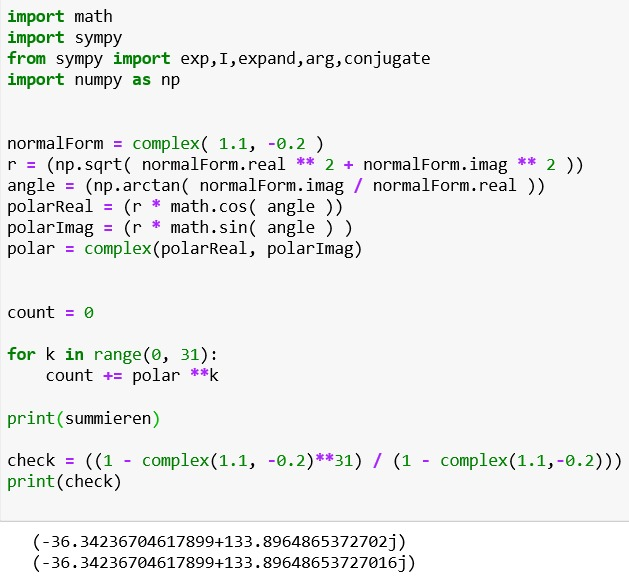
\includegraphics[width=12cm,height=10cm]{Capture}
\end{center}
\begin{center}
\bigskip
\bigskip
\bigskip
\LARGE
 \textbf{Aufgabe 3} 
\bigskip
\bigskip
\end{center}
In dieser Aufgabe ist es eine Klasse "Komplex.py" vorgegeben. Das Programm erhält als Parameter das Reale und Imaginäre Teil der Komplexen Zahl. Das Programm kann die Zahlen Verknüpfen, Addieren und deren absoluten Wert berechnen.\\
\bigskip
\textbf{(a)} In der Aufgabe musste man die Klasse erweitern indem noch zwei Methoden für Multiplikation und Division implementiert werden sollten.\\
Gegeben sind die zwei Komplexe Zahlen:
$$ z\textsubscript{1} = x\textsubscript{1} + iy\textsubscript{1}$$ $$z\textsubscript{2} = x\textsubscript{2} + iy\textsubscript{2} $$
Die Multiplikation erfolgt durch umsetzen der folgender Formel: 
$$ z\textsubscript{1} * z\textsubscript{2} = ( x\textsubscript{1} + iy\textsubscript{1})( x\textsubscript{2} + iy\textsubscript{2})$$
Bei der Multiplikation wichtig zu beachten ist, dass  $i^2 = -1$.\\
\bigskip
In Python sieht unserer Code so aus:
\begin{center}
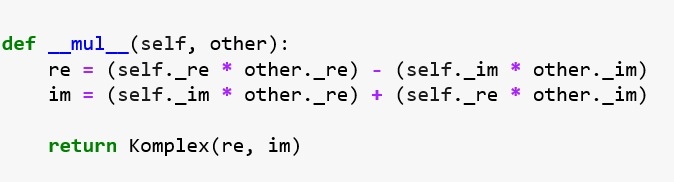
\includegraphics[width=12cm,height=4cm]{Mul}
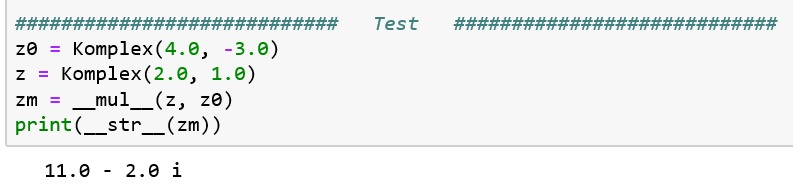
\includegraphics[width=12cm,height=4cm]{Mul2}
\end{center}
Die Division zwei komplexer Zahlen ist etwas komplizierter, wir haben die Komplexe Zahlen $z\textsubscript{1}$ und $z\textsubscript{2}$:
$$ z\textsubscript{1} = x\textsubscript{1} + iy\textsubscript{1}$$ $$z\textsubscript{2} = x\textsubscript{2} + iy\textsubscript{2} $$
Die Division erfolgt durch umsetzen der folgender Formel: 
$$\frac{z\textsubscript{1}}{ z\textsubscript{2}} = \frac{x\textsubscript{1} + iy\textsubscript{1}}{ x\textsubscript{2} + iy\textsubscript{2}} * \frac{x\textsubscript{2} - iy\textsubscript{2}}{x\textsubscript{2} - iy\textsubscript{2}} $$
\bigskip
\begin{center}
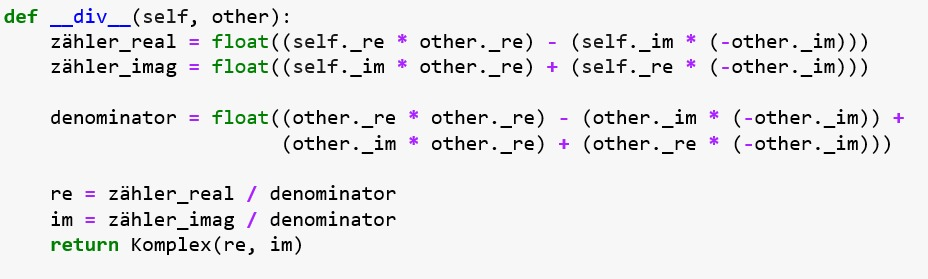
\includegraphics[width=17cm,height=5cm]{Div}
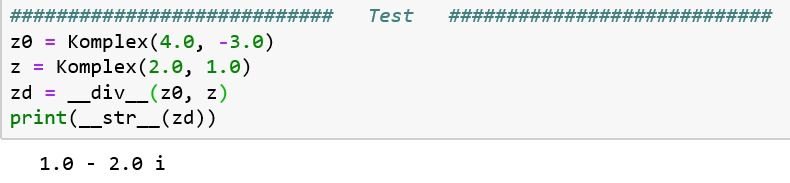
\includegraphics[width=12cm,height=5cm]{Div2}
\end{center}
\bigskip
\textbf{(b)}Und die Ergebnisse richtig ausgeben zu können haben wir uns die String Methode folgendermaßen angepasst: 
\begin{center}
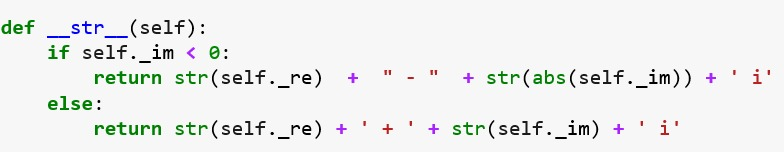
\includegraphics[width=12cm,height=4cm]{String}  
\bigskip
\end{center}
\textbf{(c)} In der letzten Teil der Aufgabe 3 haben wir die Klasse mit noch einer Methode erweitert, die eine komplexe Zahl in der exponentiellen Form ausgibt.\\
Wir haben eine Komplexe Zahl: $z = x + iy$.
Ähnlich wie in Aufgabe 1 um eine Zahl in seiner exponentiellen Form darzustellen müssen wir den Betrag und den Winkel bestimmen: $$r = \sqrt{(x^2 + y^2)}$$ \\ 
\begin{center} 
und
\end{center} $$\varphi = arctan(\frac{y}{x})$$
Die Exponentialform bekommt man jetzt nur durch der Einsetzung in der Formel: 
$$z = re ^{i\varphi}$$  Und in Python programmiert:
\bigskip
\begin{center}
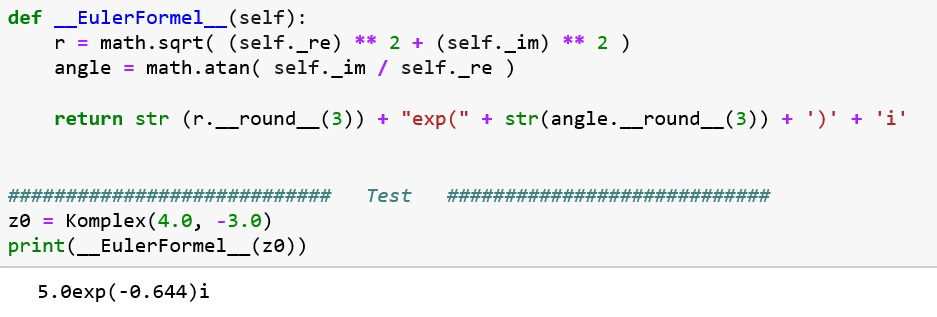
\includegraphics[width=12cm,height=5cm]{Exp}
\end{center}
\end{flushleft}
\end{document}